%! TeX program = pdflatex
\documentclass{article}
\usepackage[english]{babel}
\usepackage[utf8]{inputenc}
\usepackage{amsmath}
\usepackage{amssymb}
\usepackage{minted}
\usepackage{listings}
\usepackage{xcolor}
\usepackage{algorithm}
\usepackage{algorithmicx}
\usepackage{hyperref}
\usepackage{graphicx}
% \usepackage{natbib}
\usepackage{pgf}
% \usepackage{url}
\usepackage{algorithm}% http://ctan.org/pkg/algorithms
\usepackage{algpseudocode}% http://ctan.org/pkg/algorithmicx
% \usepackage{tikz-cd}
\usepackage{listings}
\usepackage{xcolor}
% \usepackage[colorlinks, linkcolor = blue, citecolor = magenta]{hyperref}
\usepackage{tikz}
\usetikzlibrary{positioning}
% % \usepackage{minted}
\usepackage{float}
% \usetikzlibrary{shapes, arrows, positioning}
% \lstset{ 
%     language=Python,                 % the language of the code
%     basicstyle=\ttfamily\small,      % the size of the fonts that are used for the code
%     numbers=left,                    % where to put the line-numbers
%     numberstyle=\tiny\color{gray},   % the style that is used for the line-numbers
%     stepnumber=1,                    % the step between two line-numbers. If it's 1, each line will be numbered
%     numbersep=5pt,                   % how far the line-numbers are from the code
%     backgroundcolor=\color{white},   % choose the background color. You must add \usepackage{color}
%     showspaces=false,                % show spaces adding particular underscores
%     showstringspaces=false,          % underline spaces within strings
%     showtabs=false,                  % show tabs within strings adding particular underscores
%     frame=single,                    % adds a frame around the code
%     rulecolor=\color{black},         % if not rolframe-color may be changed on line-breaks within not black text (e.g. comments (green here))
%     tabsize=4,                       % sets default tabsize to 4 spaces
%     captionpos=b,                    % sets the caption-position to bottom
%     breaklines=true,                 % sets automatic line breaking
%     breakatwhitespace=false,         % sets if automatic breaks should only happen at whitespace
%     title=\lstname,                  % show the filename of files included with \lstinputlisting; also try caption instead of title
%     keywordstyle=\color{blue},       % keyword style
%     commentstyle=\color{green},      % comment style
%     stringstyle=\color{red},         % string literal style
%     escapeinside={\%*}{*)},          % if you want to add LaTeX within your code
%     morekeywords={*,...} 
% }            % if you want to add more keywords to the rol\newenvironment{notation}
\newtheorem{remark}{Remark}
\newtheorem{definition}{Definition}
\newtheorem{property}{Property}
\newcommand{\DoParallel}[1]{\textbf{parallel do} \{#1\}}
\newcommand{\pder}[2]{\frac{\partial #1}{\partial #2}}

\title{Prototype}
\author{Pablo de Juan Vela $^{1}$ \\
        \small $^{1}$eRoots, Barcelona, Spain \\
}
\date{\today}

\usepackage[style=ieee]{biblatex}
\addbibresource{ref.bib}
\setlength{\parskip}{1em} 
\begin{document}
\maketitle

\section{Grid Definition}

We chose a modified version of the IEEE39 \cite{grids:ieee39} to demonstrate the capabilities of COLMENA. The original grid consists of 39 buses, 10 synchronous generators and 19 loads. In order to better demonstrate the capabilities of COLMENA we switch the generators to converters that can  be operated in GFM(mode) or GFL(mode). The converter in GFM mode simulates a spinning mass mirroring the behavior of a generator. We define the grid as a dynamic system that evolves over time.
\begin{figure}[h]
    \centering
    \begin{center}
        \includegraphics[width=0.8\textwidth]{plots/IEEE39 (1).png}
    \end{center}
    \caption{Your caption here}
    \label{fig:your_label}
\end{figure}

\subsection{Grid Dynamics}

\subsubsection*{Changes in the Grid's topology}

This type of changes are the ones directly affecting the connection status of an electric device. For example, switching a generator off or having a line failure.

\subsubsection*{Change in Modes}
A change in mode changes the internal definitions and states of the device. Although the power exchanges in the bus stay similar just after the change the control logic behind it can be completely changed.

\subsubsection*{Change in devices Set Points}

Here the control logic is not directly changed but some of the reference values that describe the desired steady state values. For example a reference voltage value for a converter.

\section{Roles \& Agents}


\subsection{Agents}
In the simulation we consider 6 different agents. Specifically, three of the agents are coupled to converter devices, two of them are coupled to generators and one of them is coupled to a load. At initialization, the agent receive their coupled device data from Andes. The pairings are defined before the simulation starts. We define the agents with the following hardware tags:

\begin{itemize}
    \item \textbf{Generator Compatible}
    \item \textbf{Converter Compatible}
    \item \textbf{Load Compatible}
\end{itemize}

We use this different hardware so that an agent monitoring a specific type of device can only execute the roles of compatible with that device. For example, the LoadSheddingRole only makes sense if executed in a agent thats monitoring a Load device. Therefore, adding both the hardware to the agent definition and the requirement to the role definition ensures that the roles activated in that agent are compatible with the device.

\subsection{Roles}

For this simulation use case we include different roles that participate in the frequency response. The different roles govern the agent's behaviors during the simulation. It is also through these roles that the agents can modify the grid.  



\begin{table}[h]
    \centering
    \small % Reduce font size
    \renewcommand{\arraystretch}{1.2} % Adjust row spacing
    \begin{tabular}{|p{3cm}|p{3cm}|p{4cm}|p{4cm}|} % Adjusted column widths
    \hline
    Role & Requirement & Behavior & KPI \\
    \hline
    Monitoring & None & Monitors its device's data & NA\\
    Load Shedding & Load Compatible & Reduces the device's load & $\omega \notin [\omega_{min},  \omega_max]$\\
    Automatic Secondary Response & Generator or Converter Compatible& Activates automatic response & $\omega \notin [\omega_{min},  \omega_max]$\\
    GFM & Converter Compatible & Activates the GFM Role & $\omega \notin [\omega_{min},  \omega_max]$\\
    \hline
    \end{tabular}
    \caption{Summary of Roles}
    \label{tab:roles}
\end{table}

\subsubsection*{Monitoring Role}

This role runs persistently in every agent that is paired with a physical device. When this role initializes it stores the initial values of the devices states. Then it sends periodic requests to the ANDES simulation to keep the stored values updated. Additionally, it publishes the key metrics that are important for the service in COLMENA. In this case the published metrics are the voltage of the bus the device is connected to and the generator's frequency if the agent monitors a generator. We aim to run this run continuously, this would mean syncing the stored data with a high frequency. In order to run the role continuously is executed in agents with the "EAGER" politic.  

\subsubsection*{Automatic Generation Control}

This role is activated when the frequency is seen by the agent is out of the admissible interval. This role is only compatible with devices injecting power to the grid such as generators and converters. The rol defines a PI controller with a feedback loop that adjust the power delivered by the device. The role reads the frequency value from the agent data and then sends the change in power to the device as a change of parameter.

\subsubsection*{GFM Role}

This role changes the operation mode of GFL converters to GFM to converters. It is activated when the frequency seen by the device is out of the admissible interval. When the role ends its execution the agent changes the mode of the converter back to GFM.

\subsubsection*{Load Shedding Role}

This role is engaged when the frequency is out of the admissible interval and the Automatic Generation Response has been running in a nearby generator for at least 30 seconds. When activated the agent reduces the consumed load linearly, when the role is disengaged the change is reversed.


\section{Grid Simulation}

\subsection{Andes Interaction}

The grid is simulated through the ANDES package. The Grid is initialized with the values from the power flow results. Afterwards Andes is deployed in a port where the different agents can request information from it. 

\begin{algorithm}
    \caption{Grid Simulation}
    \label{algo:COLMENAANDES}
    \begin{algorithmic}[1]
        \State Initialize grid states $x$ to $x_0$ with the Power Flow results.
        \For{agent in Agents}
            \For{device in controllable devices}
                \If{device is not controlled}
                    \State Pair agent to device
                \EndIf
            \EndFor
        \EndFor
        \While{not Stop}
            \DoParallel
                \State Receive Parameter Changes
                \State Run Simulation Online
        \EndWhile
        \State Finalize the result.
    \end{algorithmic}
\end{algorithm}

\begin{figure}[h]
    \centering
    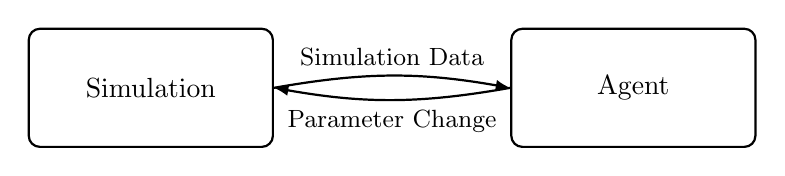
\begin{tikzpicture}[node distance=6cm and 3cm, >=latex, thick]

        % Define smaller nodes with rounded corners
        \node[draw, rectangle, rounded corners, minimum width=3.1cm, minimum height=1.5cm, align=center] (sim) {Simulation};
        \node[draw, rectangle, rounded corners, minimum width=3.1cm, minimum height=1.5cm, align=center, right=of sim] (agent) {Agent};

        % Adjusted rounded arrows with different start and end positions
        \draw[->, rounded corners] (sim.east) to[out=10, in=170] node[above, font=\small] {Simulation Data} (agent.west);
        \draw[<-, rounded corners] (sim.east) to[out=-10, in=-170] node[below, font=\small] {Parameter Change} (agent.west);
    \end{tikzpicture}
    \caption{Interaction between the simulation and agent.}
    \label{fig:sim_agent_interaction}
\end{figure}

In this use case the agents only receive data from the device their paired to and they only change the parameters of the same device. This is a constraint that comes from the agent-device pairing that we envisioned in the beginning. 

\subsection{Simulation}
The grid simulation starts from a steady-state solution that was computed before. In order to model the dynamic changes in the grid we introduce multiple changes. These changes are variable loads simulating the variability of the consumption in electric power and also line failures. These changes introduce perturbations to the grid and force the agents to respond. The objective is to showcase the different actions that the agent will perform to the grid to maintain the grid's frequency stability. The simulation runs for $70$s and observe the different transient responses compared to the simulation with just the automatic response.

\begin{table}[h]
    \centering
    \begin{tabular}{|l|c|r|}
    \hline
    Perturbation & Device & Change \\
    \hline
    Line Failure & Line 2 & Line disconnected at $t =2$s\\
    Load Reduction & Load 1 & Load increases 5\% from $t =10$s to $t =20$s\\
    Load Increase & Load 2 & Load decreases 5\% from $t =20$s to $t =30$s\\
    \hline
    \end{tabular}
    \caption{Table of non-agent induced changes in the grid}
    \label{tab:example}
\end{table}

\subsection*{Results}

\end{document}